\documentclass[conference]{IEEEtran}

\usepackage{iftex}
\ifPDFTeX
  \usepackage[utf8]{inputenc}
  \usepackage[T1]{fontenc}
\else
  \usepackage{fontspec}
  \setmainfont{texgyretermes}[
    Extension = .otf,
    UprightFont = *-regular,
    BoldFont = *-bold,
    ItalicFont = *-italic,
    BoldItalicFont = *-bolditalic]
\fi
\usepackage[brazil]{babel}
\usepackage{amsmath,amssymb}
\usepackage{icomma}
\usepackage{graphicx}
\usepackage{booktabs}
\usepackage{multirow}
\usepackage{adjustbox}
\usepackage{cite}
\usepackage{url}
\usepackage{balance}

\graphicspath{{figuras/}}
\newcommand{\ieeecaptions}{%
  \renewcommand{\abstractname}{Abstract}%
  \renewcommand{\refname}{References}%
  \renewcommand{\figurename}{Fig.}%
}
\addto\captionsbrazil{\ieeecaptions}
\AtBeginDocument{\ieeecaptions}

\begin{document}

\title{Prompt Ensembling na Classificação Zero-Shot do CLIP sob Mudança de Domínio: um Estudo Pareado com 30 Simulações}

\author{\IEEEauthorblockN{Silvio Fittipaldi}
\IEEEauthorblockA{CESAR School\\
Disciplina de Inteligência Artificial\\
Recife, Brasil\\
sfm@cesar.school}
\and
\IEEEauthorblockN{Bernardo Heuer}
\IEEEauthorblockA{CESAR School\\
Disciplina de Inteligência Artificial\\
Recife, Brasil\\
bchg@cesar.school}
\and
\IEEEauthorblockN{Rodrigo Nunes}
\IEEEauthorblockA{CESAR School\\
Disciplina de Inteligência Artificial\\
Recife, Brasil\\
rbnm@cesar.school}}

\maketitle

\begin{abstract}
Modelos de fundação multimodais como o CLIP permitem classificar imagens sem treinamento específico, bastando descrever as classes em linguagem natural. Como a classificação depende do texto usado para construir os protótipos de classe, a estratégia de formulação dos prompts é uma variável que pode alterar o desempenho, sobretudo quando as imagens de teste diferem da distribuição de pré-treinamento. Este trabalho compara duas estratégias de inferência textual no CLIP com backbone ViT-B/32: um prompt único (\textit{``a photo of a \{classe\}''}) e o Prompt Ensembling, que calcula a média L2-normalizada dos embeddings de oito templates. A avaliação usa o conjunto de teste do CIFAR-100 submetido a quatro tipos de mudança de domínio sintética (ruído gaussiano, desfoque, escala de cinza com baixo contraste e esboço) em 30 simulações pareadas de 500 imagens estratificadas. O Prompt Ensembling elevou a acurácia Top-1 média de 28,21\% para 28,63\% (diferença de +0,41 ponto percentual, IC 95\% [0,08; 0,74]). O teste de Shapiro-Wilk não rejeitou a normalidade das diferenças ($p = 0{,}174$) e o teste t pareado indicou diferença significativa ($t(29) = 2{,}554$; $p = 0{,}0162$; $d_z = 0{,}47$). O F1-Score Macro seguiu o mesmo padrão ($p = 0{,}0066$). O ganho é estatisticamente consistente, mas pequeno em termos absolutos, e não altera o custo de inferência por imagem, pois o ensemble é computado uma única vez na construção do classificador.
\end{abstract}

\begin{IEEEkeywords}
CLIP, Vision Transformer, classificação zero-shot, prompt ensembling, mudança de distribuição, modelos de fundação.
\end{IEEEkeywords}

\section{Introdução}

Durante a última década, a visão computacional foi dominada por redes neurais convolucionais (CNNs) treinadas de forma supervisionada para uma tarefa específica. Nesse paradigma especialista, cada novo conjunto de classes exige coleta e rotulação de dados e um novo ciclo de treinamento ou ajuste fino. O modelo resultante aprende um conjunto fechado de categorias e tende a perder desempenho quando a distribuição das imagens de teste se afasta da distribuição de treinamento.

Bommasani \textit{et al.}~\cite{bommasani2021} chamam de \textit{modelos de fundação} os modelos treinados em larga escala com dados amplos, em geral com auto-supervisão, e que depois são adaptados a muitas tarefas. Duas contribuições tornaram esse paradigma viável em visão. A primeira é o Vision Transformer (ViT)~\cite{dosovitskiy2020}, que aplica o encoder Transformer, originalmente proposto para texto, a uma sequência de patches da imagem, dispensando o viés indutivo das convoluções. A segunda é o CLIP~\cite{radford2021}, que treina conjuntamente um encoder de imagem e um encoder de texto com um objetivo contrastivo sobre 400 milhões de pares imagem-texto coletados da web. Como imagem e texto passam a habitar o mesmo espaço latente, qualquer conjunto de classes pode ser reconhecido sem treinamento adicional: basta escrever uma frase para cada classe e escolher a mais similar à imagem.

Essa flexibilidade desloca parte do problema para o texto. Radford \textit{et al.}~\cite{radford2021} observaram que o nome isolado da classe produz resultados inferiores a frases contextualizadas e que a média de embeddings de vários templates, chamada \textit{Prompt Ensembling}, trouxe ganho adicional de cerca de 3,5 pontos percentuais no ImageNet em relação ao prompt padrão único. Resta saber se esse ganho se mantém, e com que consistência estatística, quando as imagens sofrem mudança de domínio.

Este trabalho investiga essa questão com um protocolo pareado de 30 simulações sobre o CIFAR-100 com degradações sintéticas controladas. As contribuições são: (i) um pipeline reprodutível de classificação zero-shot com o CLIP ViT-B/32; (ii) a comparação entre prompt único e Prompt Ensembling com teste de hipótese escolhido automaticamente a partir da normalidade das diferenças; e (iii) uma análise do efeito por tipo de degradação e do custo computacional de cada estratégia.

\section{Fundamentação Teórica e Metodologia}

\subsection{Técnica A: Vision Transformer (ViT-B/32)}

O ViT~\cite{dosovitskiy2020} divide uma imagem $\mathbf{x} \in \mathbb{R}^{H \times W \times C}$ em $N = HW/P^2$ patches de lado $P$. No ViT-B/32, com entrada de $224 \times 224$ e $P = 32$, resultam $N = 49$ patches. Cada patch é achatado e projetado linearmente por uma matriz $\mathbf{E}$, e um token aprendível $\mathbf{x}_{\text{cls}}$ é concatenado no início da sequência:
\begin{equation}
\mathbf{z}_0 = [\mathbf{x}_{\text{cls}};\, \mathbf{x}_p^1\mathbf{E};\, \dots;\, \mathbf{x}_p^N\mathbf{E}] + \mathbf{E}_{\text{pos}},
\end{equation}
em que $\mathbf{E}_{\text{pos}}$ codifica a posição. A sequência de 50 tokens atravessa 12 camadas Transformer com dimensão oculta 768 e 12 cabeças de atenção. A saída correspondente ao token \texttt{[CLS]} na última camada, $\mathbf{z}_L^0$, resume a imagem inteira. No CLIP, esse vetor é normalizado e projetado por uma matriz $\mathbf{W}_v$ para o espaço conjunto de 512 dimensões, formando o embedding visual $\mathbf{v} = \mathbf{W}_v\,\mathrm{LN}(\mathbf{z}_L^0)$.

\subsection{Técnica B: alinhamento multimodal com o CLIP}

O CLIP~\cite{radford2021} combina o encoder visual $f(\cdot)$ descrito acima com um encoder de texto Transformer $g(\cdot)$, que produz o embedding de uma frase a partir do token de fim de sequência. Durante o pré-treinamento, em um lote de $B$ pares, a matriz de similaridades $s_{ij} = \tau \cos(\mathbf{v}_i, \mathbf{t}_j)$ é otimizada com entropia cruzada simétrica para que cada imagem seja mais similar ao seu próprio texto do que aos outros $B-1$ textos. A escala $\tau$, inverso de uma temperatura, é aprendida e vale 100 no modelo usado. A similaridade de cosseno é
\begin{equation}
\cos(\mathbf{v}, \mathbf{w}) = \frac{\mathbf{v}^\top \mathbf{w}}{\lVert \mathbf{v} \rVert_2\, \lVert \mathbf{w} \rVert_2}.
\end{equation}

Na classificação zero-shot com $K$ classes, cada classe $c$ é representada por um protótipo textual $\mathbf{w}_c$ e a probabilidade estimada é
\begin{equation}
p(y = c \mid \mathbf{x}) = \frac{\exp\big(\tau \cos(\mathbf{v}, \mathbf{w}_c)\big)}{\sum_{j=1}^{K} \exp\big(\tau \cos(\mathbf{v}, \mathbf{w}_j)\big)},
\end{equation}
com predição $\hat{y} = \arg\max_c \cos(\mathbf{v}, \mathbf{w}_c)$. Como $\tau > 0$ e o softmax é monotônico, a temperatura não altera a classe predita.

\subsection{Técnica C: estratégia de inferência textual}

A variável experimental é a forma de construir $\mathbf{w}_c$. Dado um conjunto de templates $\{t_1, \dots, t_T\}$, cada embedding textual é normalizado, $\mathbf{w}_{c,k} = g(t_k(c)) / \lVert g(t_k(c)) \rVert_2$, e o protótipo é
\begin{equation}
\mathbf{w}_c = \frac{\frac{1}{T}\sum_{k=1}^{T} \mathbf{w}_{c,k}}{\left\lVert \frac{1}{T}\sum_{k=1}^{T} \mathbf{w}_{c,k} \right\rVert_2}.
\end{equation}
No cenário de prompt único (H0), $T = 1$ com o template \textit{``a photo of a \{classe\}.''}. No Prompt Ensembling (H1), $T = 8$ com os templates \textit{a photo of a}, \textit{a blurry photo of a}, \textit{a sketch of a}, \textit{a low contrast photo of a}, \textit{a cropped photo of a}, \textit{a bright photo of a}, \textit{a dark photo of a} e \textit{a painting of a}, todos seguidos do nome da classe. A média no espaço normalizado funciona como um centróide de várias descrições da mesma classe e reduz a dependência de uma formulação específica. Os protótipos são calculados uma única vez; por isso, o custo por imagem na inferência é o mesmo nas duas estratégias.

\subsection{Dados e mudança de domínio}

Foi usado o conjunto de teste do CIFAR-100, com 10.000 imagens de $32 \times 32$ pixels distribuídas igualmente entre 100 classes. Os nomes das classes foram usados como estão, trocando sublinhados por espaços (por exemplo, \textit{aquarium fish}). Para simular a mudança de domínio, cada imagem recebeu um entre quatro tipos de degradação, atribuídos de forma balanceada dentro de cada classe (2.500 imagens por tipo) com semente fixa: (i) ruído gaussiano aditivo com $\sigma = 0{,}08$; (ii) desfoque gaussiano com núcleo $5 \times 5$ e $\sigma = 0{,}7$; (iii) conversão para escala de cinza com contraste reduzido a 40\%; e (iv) esboço sintético, obtido pela magnitude do gradiente de Sobel invertida, que produz traços escuros sobre fundo branco. As intensidades foram fixadas em níveis moderados antes da execução e não foram ajustadas com base nos resultados. As degradações são aplicadas na resolução nativa, e a imagem é então ampliada para $224 \times 224$ por interpolação bicúbica e normalizada com as estatísticas do CLIP. O ruído usa um gerador semeado pelo índice da imagem, de modo que cada imagem é idêntica em todas as rodadas e nos dois cenários. A Fig.~\ref{fig:exemplos} mostra exemplos.

\begin{figure}[!t]
\centering
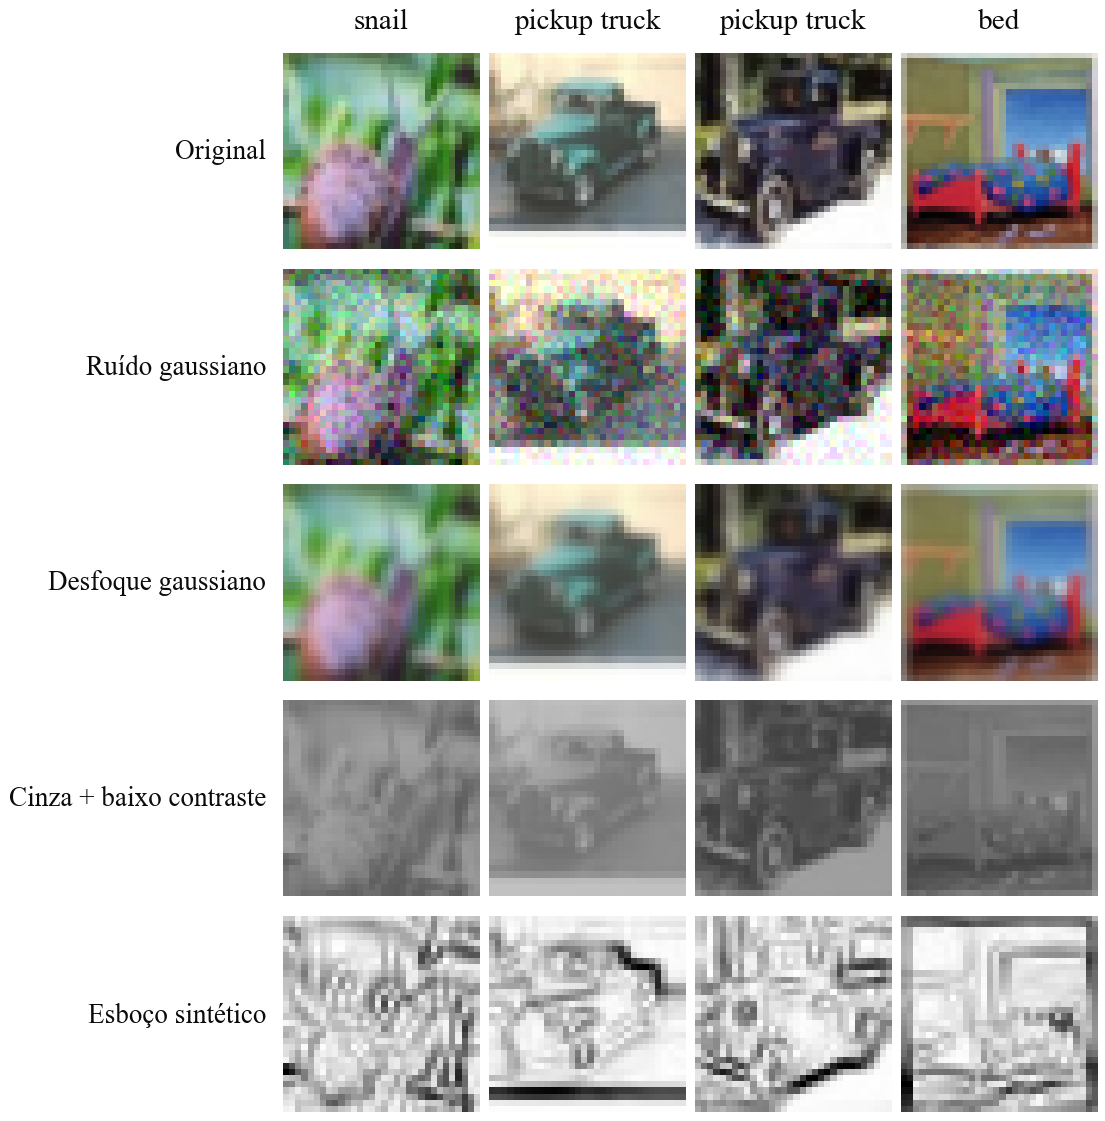
\includegraphics[width=0.8\columnwidth]{fig0_exemplos_shift.png}
\caption{Exemplos do conjunto de teste do CIFAR-100 e das quatro mudanças de domínio aplicadas na resolução nativa de $32 \times 32$.}
\label{fig:exemplos}
\end{figure}

\subsection{Hipóteses}

Seja $\Delta_i = \mathrm{Acc}_i^{\mathrm{H1}} - \mathrm{Acc}_i^{\mathrm{H0}}$ a diferença de acurácia Top-1 na rodada $i$ e $\mu_\Delta$ sua média populacional. As hipóteses são
\begin{align}
H_0&: \mu_\Delta = 0, \\
H_1&: \mu_\Delta \neq 0.
\end{align}
$H_0$ afirma que o Prompt Ensembling não altera a acurácia zero-shot sob mudança de domínio. O teste bilateral foi escolhido por ser mais conservador que o unilateral e por permitir detectar também uma eventual piora. O F1-Score Macro e os tempos de execução foram analisados com o mesmo procedimento, como métricas secundárias.

\subsection{Protocolo experimental e análise estatística}

Foram executadas 30 simulações, com a semente $i$ variando de 1 a 30. Em cada rodada, 5 imagens por classe foram sorteadas sem reposição com a semente $i$, totalizando 500 imagens. Os dois cenários foram avaliados exatamente sobre as mesmas imagens, o que caracteriza um delineamento pareado. Para evitar viés de ordem nas medidas de tempo, H0 foi executado primeiro nas sementes ímpares e H1 primeiro nas pares, e uma rodada completa de aquecimento com semente 0 foi descartada. Em cada rodada foram registrados a acurácia Top-1, o F1-Score Macro sobre as 100 classes, o tempo médio de inferência por imagem (codificação visual, similaridade e $\arg\max$) e o tempo de construção do classificador textual.

A normalidade de $\Delta$ foi verificada com o teste de Shapiro-Wilk. Quando $p > 0{,}05$, aplicou-se o teste t de Student pareado; caso contrário, o teste de postos sinalizados de Wilcoxon. O nível de significância adotado foi $\alpha = 0{,}05$. O tamanho do efeito foi medido pelo $d$ de Cohen para amostras pareadas, $d_z = \bar{\Delta} / s_\Delta$, e o intervalo de confiança de 95\% da diferença média foi calculado pela distribuição t com 29 graus de liberdade.

O experimento foi implementado em Python com PyTorch, Hugging Face Transformers, scikit-learn e SciPy, usando o modelo pré-treinado \path{openai/clip-vit-base-patch32}. A execução foi feita em CPU (processador Intel, 14 threads), sem cálculo de gradientes e com lotes de 128 imagens. Uma segunda execução completa do notebook reproduziu de forma idêntica todas as acurácias e valores de F1, o que confirma o determinismo do pipeline; apenas os tempos variam entre execuções. Os resultados brutos das 30 rodadas e o resumo estatístico acompanham o código em arquivos CSV e JSON.

\section{Resultados e Discussão}

\subsection{Desempenho de classificação}

A Tabela~\ref{tab:resultados} resume as 30 rodadas. A acurácia Top-1 média passou de 28,21\% com prompt único para 28,63\% com Prompt Ensembling, e o F1-Score Macro passou de 27,59\% para 28,07\%. Esses valores ficam muito abaixo do desempenho zero-shot relatado para o CLIP em imagens sem degradação~\cite{radford2021}, o que confirma que as transformações aplicadas produzem uma mudança de domínio severa.

\begin{table*}[!t]
\centering
\caption{Estatísticas descritivas e testes pareados nas 30 simulações (500 imagens por rodada). Acurácia e F1 em \%; $\Delta$ = H1 $-$ H0.}
\label{tab:resultados}
\footnotesize
\setlength{\tabcolsep}{3.5pt}
\begin{adjustbox}{max width=\textwidth}
\begin{tabular}{lcccccccc}
\toprule
\multirow{2}{*}{Métrica} & \multicolumn{2}{c}{Média $\pm$ DP} & \multicolumn{2}{c}{Mediana [IQR]} & \multirow{2}{*}{$\bar{\Delta}$ [IC 95\%]} & Shapiro-Wilk & \multirow{2}{*}{Teste e $p$-valor} & \multirow{2}{*}{$d_z$} \\
\cmidrule(lr){2-3} \cmidrule(lr){4-5}
 & H0 & H1 & H0 & H1 & & $p$ ($\Delta$) & & \\
\midrule
Acurácia Top-1 & 28,21 $\pm$ 2,14 & 28,63 $\pm$ 2,04 & 28,20 [2,30] & 28,70 [2,60] & +0,41 [0,08; 0,74] & 0,174 & t pareado, $p = 0{,}0162$ & 0,47 \\
F1-Score Macro & 27,59 $\pm$ 2,02 & 28,07 $\pm$ 2,02 & 27,71 [2,24] & 28,11 [2,93] & +0,48 [0,14; 0,82] & 0,192 & t pareado, $p = 0{,}0066$ & 0,53 \\
Inferência (ms/img) & 24,02 $\pm$ 1,51 & 24,03 $\pm$ 1,61 & 23,95 [1,63] & 23,58 [2,01] & +0,01 [$-$0,34; 0,35] & 0,497 & t pareado, $p = 0{,}964$ & 0,01 \\
Classif. textual (s) & 0,29 $\pm$ 0,22 & 2,14 $\pm$ 0,14 & 0,24 [0,03] & 2,15 [0,19] & +1,85 [1,76; 1,94] & $<$0,001 & Wilcoxon, $p = 1{,}9 \times 10^{-9}$ & 7,89 \\
\bottomrule
\end{tabular}
\end{adjustbox}
\end{table*}

O teste de Shapiro-Wilk aplicado às diferenças de acurácia resultou em $W = 0{,}9505$ e $p = 0{,}174$, sem evidência contra a normalidade. Pela regra pré-definida, aplicou-se o teste t pareado, que resultou em $t(29) = 2{,}554$ e $p = 0{,}0162$. Como $p < \alpha = 0{,}05$, rejeita-se $H_0$: há evidência de que o Prompt Ensembling altera a acurácia, e o sinal positivo da diferença média indica que essa alteração é uma melhora. O intervalo de confiança de 95\% para a diferença média, $[0{,}08; 0{,}74]$ ponto percentual, não contém o zero, o que é coerente com o teste. O $p$-valor deve ser lido como a probabilidade de observar uma diferença média tão grande quanto a observada se não houvesse efeito algum; ele não mede a magnitude do ganho nem a probabilidade de $H_1$ ser verdadeira. O F1-Score Macro levou à mesma conclusão ($W = 0{,}9521$, $p_{\mathrm{SW}} = 0{,}192$; $t(29) = 2{,}925$; $p = 0{,}0066$; $d_z = 0{,}53$), o que indica que o ganho não está concentrado em poucas classes.

A Fig.~\ref{fig:box} mostra a distribuição das 30 acurácias por cenário. A variação entre rodadas (desvio padrão de cerca de 2 pontos percentuais) é muito maior que a diferença entre os cenários, de modo que uma comparação não pareada dificilmente detectaria o efeito. O pareamento remove a variabilidade causada pela composição de cada amostra, e é isso que torna o ganho de 0,41 ponto percentual detectável. A Fig.~\ref{fig:barras} apresenta lado a lado as médias e os desvios padrão das duas métricas de classificação.

\begin{figure}[!t]
\centering
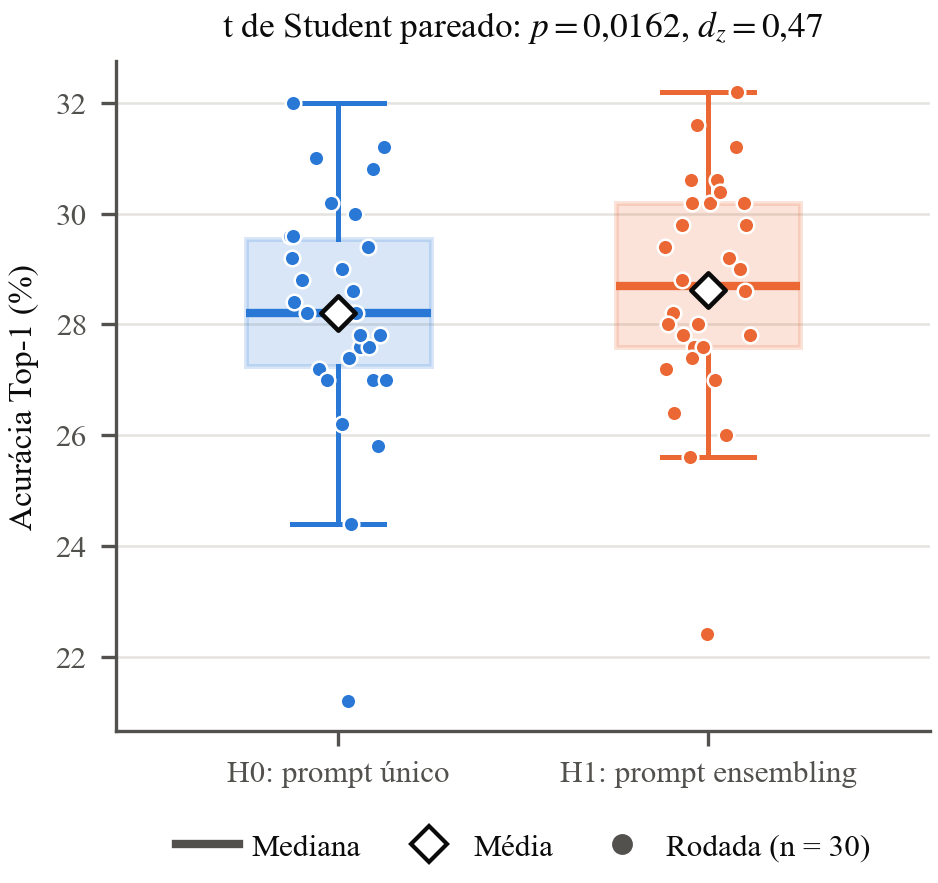
\includegraphics[width=\columnwidth]{fig1_comparacao_acuracia.png}
\caption{Acurácia Top-1 nas 30 simulações. Caixas indicam mediana e IQR, pontos representam rodadas individuais e losangos marcam a média.}
\label{fig:box}
\end{figure}

\begin{figure}[!t]
\centering
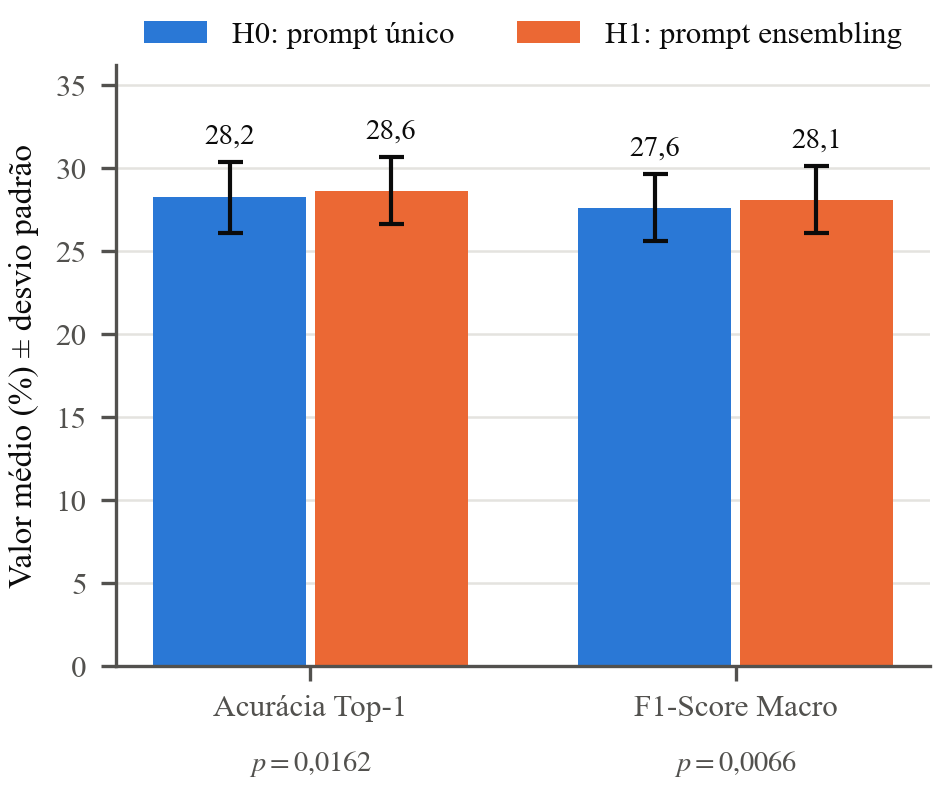
\includegraphics[width=\columnwidth]{fig3_tradeoff_metricas.png}
\caption{Acurácia Top-1 e F1-Score Macro médios com barras de desvio padrão nas 30 simulações. Os $p$-valores dos testes pareados aparecem abaixo de cada métrica.}
\label{fig:barras}
\end{figure}

\begin{figure*}[!t]
\centering
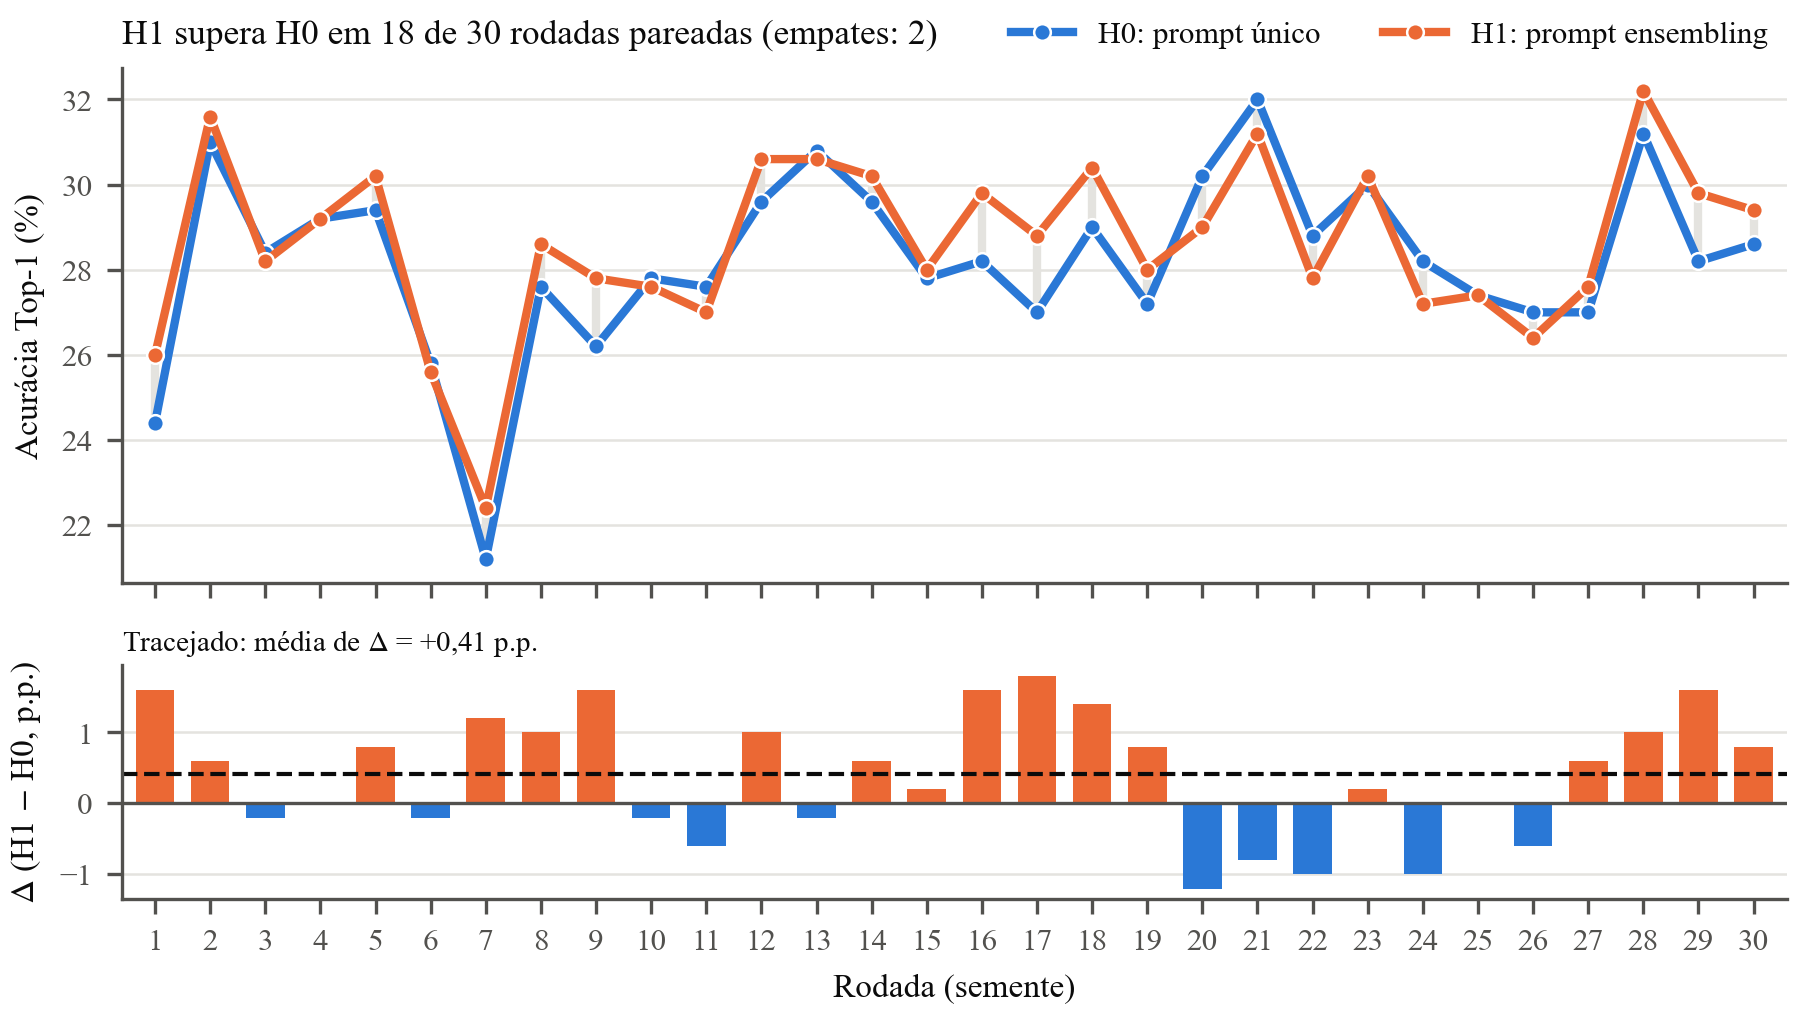
\includegraphics[width=\textwidth]{fig2_evolucao_pareada.png}
\caption{Acurácia Top-1 por rodada nos dois cenários (acima) e diferença pareada $\Delta_i$ em pontos percentuais (abaixo). As mesmas 500 imagens são usadas por H0 e H1 em cada semente.}
\label{fig:pareada}
\end{figure*}

A Fig.~\ref{fig:pareada} detalha o comportamento rodada a rodada. O Prompt Ensembling superou o prompt único em 18 das 30 rodadas, empatou em 2 e perdeu em 10, com diferenças entre $-1{,}2$ e $+1{,}8$ ponto percentual. A superioridade é, portanto, consistente em média, mas não uniforme. Pelas convenções usuais de Cohen, $d_z = 0{,}47$ corresponde a um efeito entre pequeno e médio. É preciso cuidado com essa leitura, porque $d_z$ é calculado sobre a dispersão das diferenças pareadas, que é pequena; em termos absolutos, o ganho representa cerca de 2 imagens corretas a mais em cada 500.

\subsection{Efeito por tipo de mudança de domínio}

A Tabela~\ref{tab:shift} desagrega a acurácia média pelo tipo de degradação. O desfoque foi a transformação menos prejudicial e o esboço sintético a mais severa, com acurácia próxima de 12\%. O maior ganho do Prompt Ensembling ocorreu nas imagens em escala de cinza com baixo contraste (+0,88 ponto percentual), justamente o domínio descrito literalmente por um dos templates (\textit{a low contrast photo of a}). Já o template \textit{a sketch of a} trouxe ganho pequeno nas imagens de esboço (+0,25). Uma explicação plausível é que bordas extraídas de imagens de $32 \times 32$ pixels perdem informação demais para que a descrição textual compense, e o problema passa a ser a ausência de sinal visual, e não o desalinhamento entre texto e imagem.

\begin{table}[!t]
\centering
\caption{Acurácia Top-1 média (\%) por tipo de mudança de domínio}
\label{tab:shift}
\begin{tabular}{lccc}
\toprule
Mudança de domínio & H0 & H1 & $\Delta$ (p.p.) \\
\midrule
Ruído gaussiano & 22,16 & 22,34 & +0,18 \\
Desfoque gaussiano & 46,73 & 47,08 & +0,36 \\
Cinza e baixo contraste & 31,63 & 32,51 & +0,88 \\
Esboço sintético & 12,05 & 12,30 & +0,25 \\
\bottomrule
\end{tabular}
\end{table}

\subsection{Custo computacional}

O tempo médio de inferência por imagem foi de 24,02 ms com prompt único e 24,03 ms com Prompt Ensembling. As diferenças pareadas foram compatíveis com a normalidade (Shapiro-Wilk, $p = 0{,}497$), e o teste t pareado não indicou diferença ($t(29) = 0{,}045$; $p = 0{,}964$; $d_z = 0{,}01$). O resultado era esperado, pois as duas estratégias executam exatamente o mesmo encoder visual e diferem apenas nos valores da matriz de protótipos. O custo do ensemble aparece na construção do classificador, que codifica 800 prompts em vez de 100: em média 2,14 s contra 0,29 s. Nesse caso as diferenças não seguiram distribuição normal (Shapiro-Wilk, $p < 0{,}001$), em parte por um pico de 1,46 s em uma rodada de H0, e a regra de decisão selecionou o teste de Wilcoxon ($p = 1{,}9 \times 10^{-9}$, com H1 mais lento nas 30 rodadas). Esse custo é pago uma única vez por conjunto de classes e se torna desprezível quando o classificador é reutilizado.

\subsection{Limitações}
\balance

Alguns fatores restringem a generalização dos resultados. Primeiro, as 30 amostras são sorteadas do mesmo conjunto de 10.000 imagens; as rodadas compartilham imagens e não são totalmente independentes, o que tende a subestimar a variância entre amostras de uma população maior. Segundo, as degradações são sintéticas e aplicadas a imagens de baixa resolução ampliadas para $224 \times 224$, situação distante das fotografias da web usadas no pré-treinamento. Terceiro, parte dos templates de H1 descreve explicitamente as degradações aplicadas (desfocado, esboço, baixo contraste), o que pode favorecer o ensemble neste cenário específico; um controle com templates neutros ajudaria a separar o efeito da média de prompts do efeito de descrever o domínio. Por fim, foi avaliado apenas um modelo (ViT-B/32), e as medições de tempo foram feitas em CPU.

Há ainda limitações do próprio CLIP. O modelo aprende associações globais entre imagem e texto e tem dificuldade com composicionalidade, como relacionar atributos ao objeto correto ou contar objetos, pois o objetivo contrastivo pode ser satisfeito com uma representação próxima de um saco de palavras. O pré-treinamento com pares coletados da web também transfere vieses desses dados: conceitos frequentes na internet são mais bem representados, e nomes de classe ambíguos (\textit{mouse}, \textit{ray}, \textit{plain}) podem ser interpretados pelo sentido mais comum na web, e não pelo sentido pretendido no dataset. Radford \textit{et al.}~\cite{radford2021} e Bommasani \textit{et al.}~\cite{bommasani2021} discutem como esses vieses se propagam para todas as aplicações derivadas de um modelo de fundação.

\section{Conclusão}

Este trabalho comparou duas estratégias de inferência textual para classificação zero-shot com o CLIP ViT-B/32 sob mudança de domínio. Em 30 simulações pareadas sobre o CIFAR-100 degradado, o Prompt Ensembling com oito templates aumentou a acurácia Top-1 de 28,21\% para 28,63\% e o F1-Score Macro de 27,59\% para 28,07\%. As diferenças foram estatisticamente significativas pelo teste t pareado ($p = 0{,}0162$ e $p = 0{,}0066$), e a hipótese nula foi rejeitada ao nível de 5\%. O ganho absoluto, porém, é pequeno e não ocorre em todas as rodadas: H1 venceu em 18 das 30.

Do ponto de vista prático, o Prompt Ensembling é uma melhoria de baixo risco, pois não exige treinamento, não altera o custo de inferência por imagem e acrescenta apenas um custo fixo na construção do classificador. Por outro lado, a estratégia não compensa a perda de desempenho causada pela mudança de domínio, que reduziu a acurácia a menos de 30\%. Trabalhos futuros podem incluir templates neutros como controle, mudanças de domínio naturais, modelos maiores como ViT-B/16 e ViT-L/14, e métodos que adaptam os prompts com poucos exemplos rotulados.

\begin{thebibliography}{1}

\bibitem{dosovitskiy2020}
A.~Dosovitskiy, L.~Beyer, A.~Kolesnikov, D.~Weissenborn, X.~Zhai, T.~Unterthiner, M.~Dehghani, M.~Minderer, G.~Heigold, S.~Gelly, J.~Uszkoreit, and N.~Houlsby, ``An image is worth 16x16 words: Transformers for image recognition at scale,'' \textit{arXiv preprint arXiv:2010.11929}, 2020. Also in \textit{Proc. Int. Conf. Learning Representations (ICLR)}, 2021.

\bibitem{radford2021}
A.~Radford, J.~W. Kim, C.~Hallacy, A.~Ramesh, G.~Goh, S.~Agarwal, G.~Sastry, A.~Askell, P.~Mishkin, J.~Clark, G.~Krueger, and I.~Sutskever, ``Learning transferable visual models from natural language supervision,'' in \textit{Proc. 38th Int. Conf. Machine Learning (ICML)}, PMLR, vol.~139, 2021, pp.~8748--8763.

\bibitem{bommasani2021}
R.~Bommasani \textit{et al.}, ``On the opportunities and risks of foundation models,'' \textit{arXiv preprint arXiv:2108.07258}, 2021.

\end{thebibliography}

\end{document}
